\documentclass[a4paper, 11pt, english]{article}
	\usepackage{tabu, listings, babel, blindtext, graphicx, amsmath, mathtools}
	\author{Kim Rune Solstad, TDT4200, NTNU}
	\title{Assignment 2, MPI}

	\lstset{language=c}

\begin{document}
\maketitle
\section*{Problem 1}
\subsection{a)}
Explain the difference between MPI\_Send(), MPI\_Isend() and MPI\_Ssend().
\\
\\
The three functions mentioned are mpi send functions with different modes. Different modes will give the program different guarantees. The four send modes in MPI are:
\begin{enumerate}
	\item Standard
	\item Synchronized
	\item Bufferred
	\item Ready
\end{enumerate}

MPI\_Send() is the standard mode. It will send the message absent any hazzles or guaranties. MPI\_Ssend() is the send function that belongs to the synchronized mode. MPI\_Ssend() will complete the transmission when it has been received at the other end. All of these functions have non-blocking alternatives. By blocking, we mean that execution will be suspended until the message buffer is safe to use. MPI\_Isend is the non-blocking alternative to MPI\_Send(). 
\subsection{b)}
What is a communicator in MPI? What is the purpose of a cartesian communicator?
\\\\
A communicator is a collection of processes that can send messages to each other. The cartesian communicator has a topology of a multi-dimensional array.

\section*{Problem 2}
\subsection*{a)}
\subsection*{The ring interconnect}
	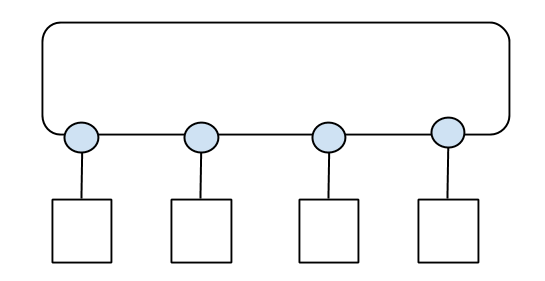
\includegraphics[width=0.8\textwidth]{ring.png}
\subsection*{The hypercube interconnect}
	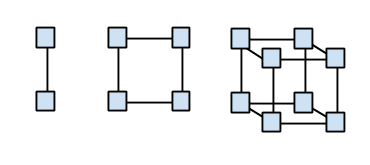
\includegraphics[width=0.8\textwidth]{hypercube.png}
	\\The picture shows a one, two and three dimensional example of a hypercube.
\subsection{The crossbar interconnect}
	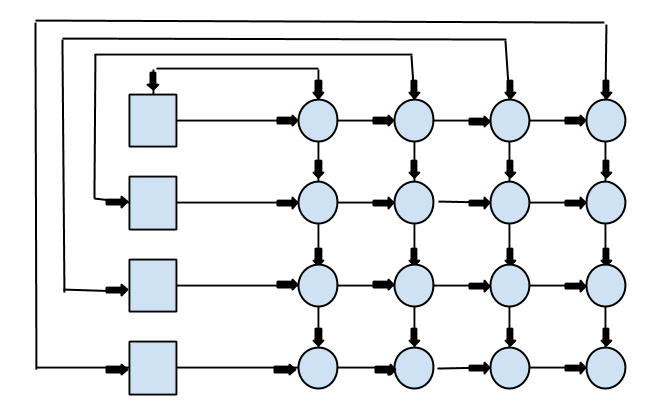
\includegraphics[width=0.8\textwidth]{crossbar.png}
\subsection*{b)}
The hypercube in dimension $n$ is made up of to hypercubes in the \begin{math}n-1\end{math} dimension. The number of processors, \begin{math}p\end{math}, in a hypercube is therefore twice the amount of processors in a hypercube of dimension \begin{math}n-1\end{math}. When making a hypercube with dimension n, the processors in the two \begin{math}n-1\end{math} hypercubes needs to be connected. This will require the same amount of connection as processors in one \begin{math}n-1\end{math} dimensional hypercube. When making a bisection of a hypercube with dimension \begin{math}n\end{math}, the bisection will be a hypercube with dimension \begin{math}n-1\end{math} wich has half the number of processors. The same amount of connections will be removed. The illustration below shows how we end up with a bisection by removing four connections from a 3-dimensional hypercube.\\
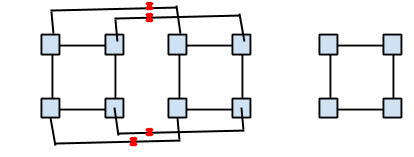
\includegraphics[width=0.8\textwidth]{bisection_width_hypercube_3d}
\section*{Problem 3}
$S$: Speed up
$p$: Amount of processors
$\alpha$: serial fraction
\subsection*{a)}
Amdahl's law:
\begin{math}
S(p) = \frac{T_{serial}} {T_{serial}(\alpha + \frac{1}{n}(1-\alpha))}
=	\frac{1}{\alpha + \frac{1}{p}(1-\alpha)}
\end{math}\\
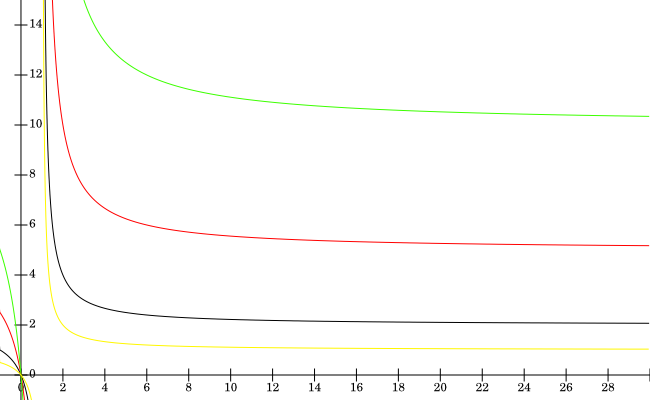
\includegraphics[width=0.8\textwidth]{p2_a}
\\black $\alpha = 0.5$ red $\alpha=0.3$ green $\alpha=0.1$ yellow $\alpha=1$
\\Best case scenario, the speed of the parallizable part is negligible.
\subsection*{b)}
Gustafson's law: 
\begin{math}
S(p) = \alpha + p(1 - \alpha)
\end{math}\\
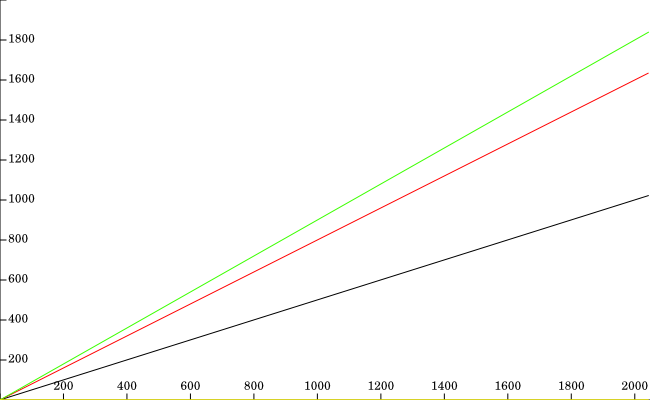
\includegraphics[width=0.8\textwidth]{p3_b}
\\black $\alpha = 0.5$ red $\alpha=0.3$ green $\alpha=0.1$ yellow $\alpha=1$
\subsection*{c)}
Gustafson's law takes into account that as the problem increases, so does the parallelizable fraction of the program. Amdahl's law takes forgranted that the serializable fraction of the program stays the same.
\subsection*{d)}


\section*{Problem 4}
\subsection*{a)}
Each of the subdomains should contain  
\begin{math}
\frac{1024^2}{64} = 16384 = 128 * 128
\end{math}
squares. The possibities are:\\
\begin{tabular}{l c r }
	x && y	\\
	\hline
	16 	&$*$& 	1024 	\\
	32 	&$*$& 	512 	\\ 
	64 	&$*$& 	256 	\\
	128 	&$*$& 	128 	\\
	256 	&$*$& 	64 	\\
	512 	&$*$& 	32 	\\
	1024 	&$*$& 	16 	\\
\end{tabular}

\subsection*{b)}


\section*{Ref}
\begin{enumerate}
	\item www.ncsa.illinois.edu/UserInfo/Resources/Hardware/CommonDoc/MessPass/MPIBlock.html
	\item Reevaluating Amdahl's law--John L. Gustafson
\end{enumerate}

\end{document}
